%%%%%%%%%%%%%%%%%%%%%%%%%%%%%%%%%%%%%%%%%%%%%%%%%%%%%%%%%%%%%%%%%%%%%%%%%%%%%%%%%%%%%%%%%%%%%%%%%%%%%%%%%%%%%%%%%%%%%%%%%%%%%%
%2345678901234567890123456789012345678901234567890123456789012345678901234567890
%        1         2         3         4         5         6         7         8

\documentclass[letterpaper, 10 pt, conference]{ieeeconf}  
% Comment this line out if you need a4paper

%\documentclass[a4paper, 10pt, conference]{ieeeconf}      
% Use this line for a4 paper

\IEEEoverridecommandlockouts       % This command is only
                                                          % needed if you want to
                                                          % use the \thanks command
\overrideIEEEmargins
% See the \addtolength command later in the file to balance the column lengths
% on the last page of the document

% The following packages can be found on http:\\www.ctan.org
\usepackage{graphics} % for pdf, bitmapped graphics files
\usepackage{epsfig} % for postscript graphics files
\usepackage{mathptmx} % assumes new font selection scheme installed
\usepackage{times} % assumes new font selection scheme installed
%\usepackage{amsmath} % assumes amsmath package installed
%\usepackage{amssymb}  % assumes amsmath package installed
\usepackage{hyperref}
\usepackage{lipsum}
\usepackage{pythonhighlight}
\usepackage{textcomp}

\title{\LARGE \bf
Generating Musical Notes and Transcription using Deep Learning$^{*}$}

\author{Varad Meru$^{\#}$% <-this % stops a space
\\ {\small Student \# 26648958}
\thanks{$^{*}$This work was done as a part of the project for the course CS 274c: Neural Networks and Deep Learning, taught in Winter 2015 by Prof. Pierre Baldi at University of California, Irvine.}% <-this % stops a space
\thanks{$^{\#}$Dept. of Computer Science, Donald Bren School of Information and Computer Science, University of California, Irvine, email: {\tt\small vmeru@ics.uci.edu}}%
}

\begin{document}
\maketitle
\thispagestyle{empty}
\pagestyle{empty}

%%%%%%%%%%%%%%%%%%%%%%%%%%%%%%%%%%%%%%%%%%%%%%%%%%%%%%%%%%%%%%%%%%%%%%%%%%%%%%%%%%%%%%%%%%%%%%%%%%%%%%%%%%%%%%%%%%%%%%%%%%%%%%
\begin{abstract}
Music has always been the most followed art form, and lot of research had gone into understanding it. In recent years, deep learning approaches for building unsupervised hierarchical representations from unlabeled data have gained significant interest. Progress in fields, such as image processing and natural language processing, has been substantial, but to my knowledge, methods on auditory data for learning representations have not been studied extensively. In this project I try to use two methods for generating music from range of musical inputs such as MIDI to complex WAV formats. I use RNN-RBMs and CDBN to explore music 
\end{abstract}
%%%%%%%%%%%%%%%%%%%%%%%%%%%%%%%%%%%%%%%%%%%%%%%%%%%%%%%%%%%%%%%
%%%%%%%%%%%%%%%%%%%%%%%%%%%%%%%%%%%%%%%%%%%%%%%%%%%%%%%%%%%%%%%
\section{Introduction}

Tasks such such as object identification in an image or completing a sentence based on the context, which humans start doing from a very early age, are very challenging for a machine to perform as the formulation of these tasks into a set of steps is very complicated. The approaches till now were focussed more on the statistical properties of the corpus and thus, the features of the data were required to be hand engineered. This gave us good results, but hand-engineering of features was extremely complicated process for very large, unstructured and complex data such as images, speech, text corpus. Recent advances in deep learning have shown huge progress in solving these problems by focusing on generating the abstract features from the data, especially in the fields of image processing and natural language processing, but not much has been done in the field of audio signals. 

This project is an attempt to understand auditory signals better using deep learning methods and using that knowledge to generate music by learning from various sources of audio signals. There are two parts of this project: Understanding the temporal dependencies in a polyphonic music using the generalization of the RTRBM, called RNN-RBM\cite{c8}, to generate music from polyphonic MIDI tones, and, apply the theory of Convolutional Deep-Belief networks\cite{c1} to learn abstract representations of the low-level description of audio signals such as STFTs and Chroma and recreating it. This work is inspired from AARON, the painter,\cite{c5} and the idea of machine doing art, which is one of the most abstract representations of human understanding, and from the work done by Tristan Jehan\cite{c4} on music synthesis using lower-level features of audio signals

Many music information retrieval (MIR) tasks depend on the extraction of low-level acoustic features. These features are usually constructed using task-dependent signal processing techniques. There are many features which are potentially useful for working with music: spectral, timbral, temporal, harmonic, etc (see \cite{c3} for a good review of features). This project tries to analyze these features and apply in the context of music synthesis. 

The remainder of the paper is organized as follows. In Sections 2, the preliminaries of the work are described. In 3 and 4, the RNN-RBM based architecture and the convolutional deep belief network (CDBN) approach to music understanding and synthesis is described. In Section 5, the datasets are described. In Section 6, I present the results on musical sequences and transcription.

%%%%%%%%%%%%%%%%%%%%%%%%%%%%%%%%%%%%%%%%%%%%%%%%%%%%%%%%%%%%%%%
%%%%%%%%%%%%%%%%%%%%%%%%%%%%%%%%%%%%%%%%%%%%%%%%%%%%%%%%%%%%%%%
\section{Preliminaries}
This section describes the preliminaries of this project. %
\subsection{Music Information Retrieval}
Music information retrieval (MIR) is an upcoming field of research and uses the knowledge from the fields of signal processing, machine learning, music and information theory. It is looking into describing the {\it bits} of the digital music in ways that facilitate searching through this abundant but latent information without structure. A survey of MIR systems can be found at \cite{c6} and \cite{c7} for reference. The most popular MIR tasks are:
\begin{itemize}
\item {\bf Fingerprinting}: finding compact representation of songs to distinct it from other songs.
\item {\bf Query by description}: description could be some text descriptors of music, or some sound input like "humming", which the system would then compare its database for similarity.
\item {\bf Music similarity}: estimating the closeness of music signals.
\item {\bf Classification}: classifying based on genre, artist, instrument, etc. 
\item {\bf Thumbnailing}: building the most "representative" audio summary of a piece of music.
\end{itemize}
There are various types of features that can be fetched form audio files. A detailed explanation of the features is described in the Appendix.

\begin{figure}[thpb]
      \centering
      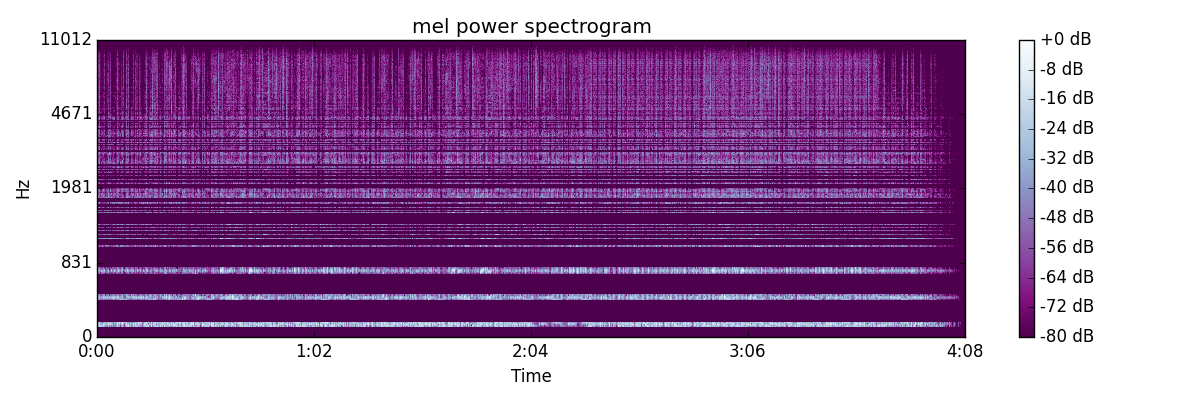
\includegraphics[scale=0.25]{mel_getlucky_3000_mels.png}
      \caption{Mel Spectrogram of a Song. (Song: Get Lucky, 2013)}
      \label{fig:mel}
\end{figure}

\begin{figure}[thpb]
      \centering
      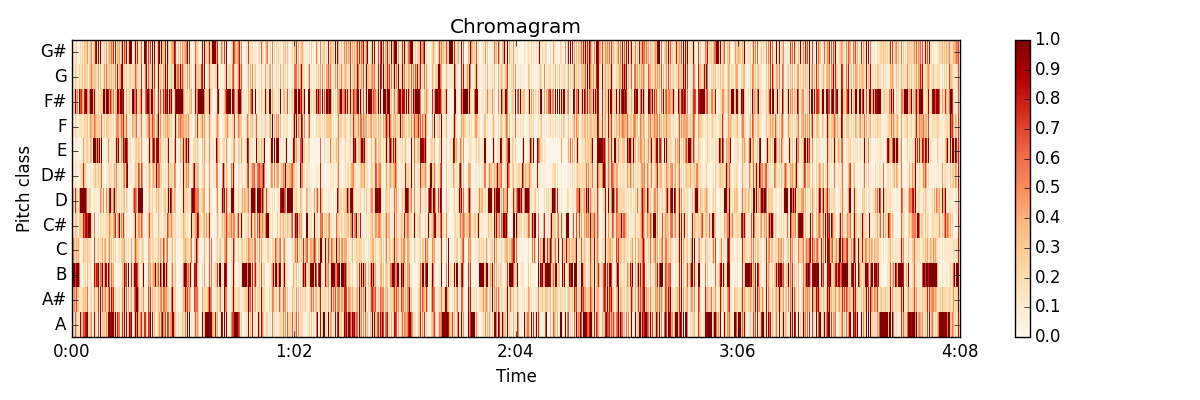
\includegraphics[scale=0.25]{chroma_get_lucky.png}
      \caption{Chroma of a Song. (Song: Get Lucky, 2013)}
      \label{fig:choma}
\end{figure}

\subsection{Musical Instrument Digital Interface (MIDI)}
MIDI is a numerical representation of music events, rather than a sampled recording like WAV or MP3. Specifically, MIDI tracks the beginning and ending of musical notes, divided into tracks where one track normally represents one instrument or voice within the musical performance. Each note in a MIDI note sequence is associated with a volume (velocity), a pitch, and a duration, and can also be modified by global track parameters such as tempo and pitch bending. Example of the MIDI transcription process can be seen in Fig. \ref{fig:midi}.
\begin{figure}[thpb]
      \centering
      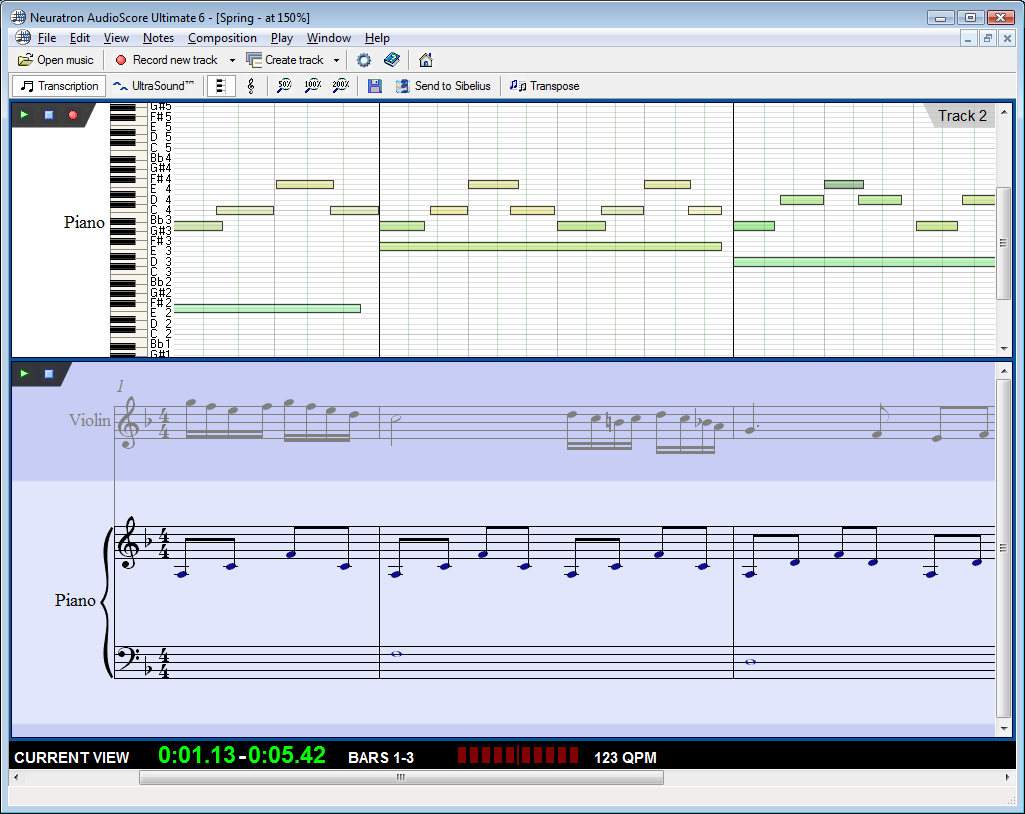
\includegraphics[scale=0.23]{trans.png}
      \caption{MIDI transcription of a sample Piano-roll, along with musical notations.}
      \label{fig:midi}
\end{figure}

\subsection{Restricted Boltzmann machines}
A Restricted Boltzmann machines(RBM) is an energy-based model where the joint probability of a given configuration of the visible vector $v$ (inputs) and the hidden vector $h$ is:
\begin{equation}
P(v,h) = \exp(-b_v^\textrm{T} v -b_v^\textrm{T} -h^\textrm{T}Wv )/Z
\end{equation}

where $b_v$, $b_h$ and $W$ are the model parameters and $Z$ is the usually intractable partition function. When the vector $v$ is given, the hidden units $h_i$ are conditionally independent of one another, and vice versa: 
\begin{equation}
P(h_i = 1 | v) = \sigma(b_h + W_v)_i
\end{equation}
\begin{equation}
P(v_j = 1 | h) = \sigma(b_v + W^\textrm{T} h)_j
\end{equation}
Where $\sigma(x) \equiv(1 + e^{-x})^{-1}$ is the logistic sigmoid function.

Inference in RBMs consists of sampling the $h_i$ given $v$, or vice versa, according to their Bernoulli distribution (given in eq. 2). Sampling $v$ can be performed efficiently by block Gibbs sampling. The gradient of the negative log likelihood of an input vector can be estimated by a single visible sample obtained from a $k$-step Gibbs chain starting $v^{(l)}$, resulting in the contrastive divergence algorithm \cite{c9}. The RBM is a generative model and its parameters can be optimized by performing stochastic gradient descent on the log-likelihood of training data. Unfortunately, the exact value is intractable. Instead, one typically uses the contrastive divergence approximation.
%
\begin{figure}[thpb]
      \centering
      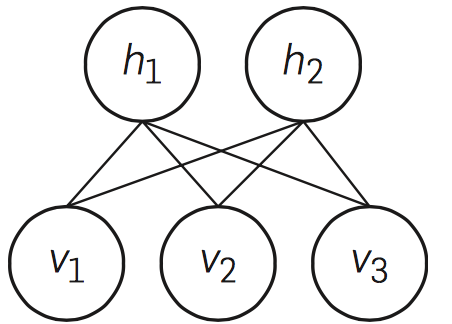
\includegraphics[scale=0.35]{rbm.png}
      \caption{RBM with three visible units (D = 3) and two hidden units (K = 2). (src: \cite{c12})}
      \label{fig:rbm}
\end{figure}

\subsection{Deep Belief Network}
The RBM is limited in what it can learn to represent. It becomes more robust when it is stacked to form a Deep Belief Network(DBN). It is a generative model consisting of many layers. An example DBN can be seen in Fig. \ref{fig:dbn}, which has three RBMs stacked. Two adjacent layers are fully connected between them, but no two units in the same layer are connected. In a DBN, each layer comprises a set of binary or real-valued units. Hinton et. al.\cite{c13} proposed an efficient algorithm for training DBNs which would greedily train each layer as an RBM using the previous layer's activations as inputs.
\begin{figure}[thpb]
      \centering
      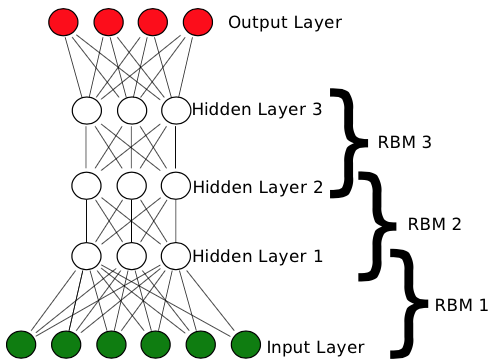
\includegraphics[scale=0.65]{dbn.png}
      \caption{DBN with three RBMs stacked. The hidden layers may not have same number of units}
      \label{fig:dbn}
\end{figure}

%%%%%%%%%%%%%%%%%%%%%%%%%%%%%%%%%%%%%%%%%%%%%%%%%%%%%%%%%%%%
%%%%%%%%%%%%%%%%%%%%%%%%%%%%%%%%%%%%%%%%%%%%%%%%%%%%%%%%%%%%
\section{The Rnn-Rbm}
The RNN-RBM\cite{c8} extends the work on the recurrent temporal RBM (RTRBM)\cite{c13}. A simple RTRBM can be seen in \ref{fig:rtrbm} which shows the unrolled version of the recurrent network. The RTRBM is a sequence of conditional RBMs (one at each step) whose parameters are time dependent and depend on the sequence history at time t. The RTRBM is formally defined by its joint probability distribution:
\begin{equation}
P(\{v^{(t)}, h^{(t)}\}) = \Pi_{t=1}^{T} P(v^{(t)}, h^{(t)} | \mathrm{A}^{(t)})
\label{eq:e1}
\end{equation}
Where $\mathrm{A}^{(t)}$ denotes the sequence history at time $t$ and is $\mathrm{A}^{(t)} \equiv \{ v^{(\tau)}, \hat{h}^{(\tau)} | \tau \textless t \}$ and $ P(v^{(t)}, h^{(t)} | \mathrm{A}^{(t)})$ is the joint probability of the $t^{\mathsf{th}}$ RBM. The RTRBM can be understood as a chain of conditional RBMs who parameters are the output of a deterministic RNN, with the constraint that the hidden units describing the conditional distributions and convey temporal information. RNNRBM is formed when a full RNN with distinct hidden units $\hat{h}^{(t)}$ with the RTRBM graphical model as shown in Fig. \ref{fig:rnnrbm}. It as the same probability distribution given in equation \ref{eq:e1}.

\begin{figure}[thpb]
      \centering
      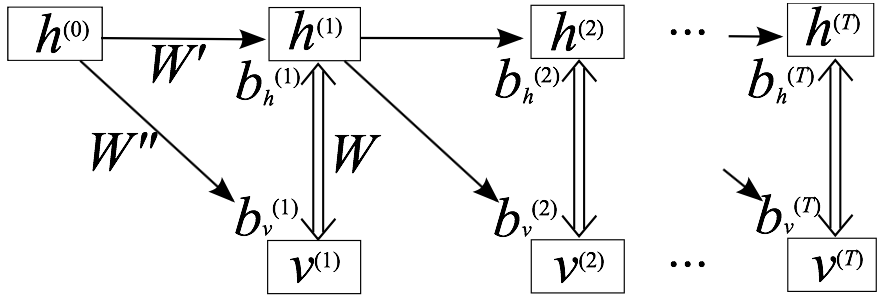
\includegraphics[scale=0.35]{rtrbm.png}
      \caption{RNN-RBM (src: \cite{c8})}
      \label{fig:rtrbm}
\end{figure}

\begin{figure}[thpb]
      \centering
      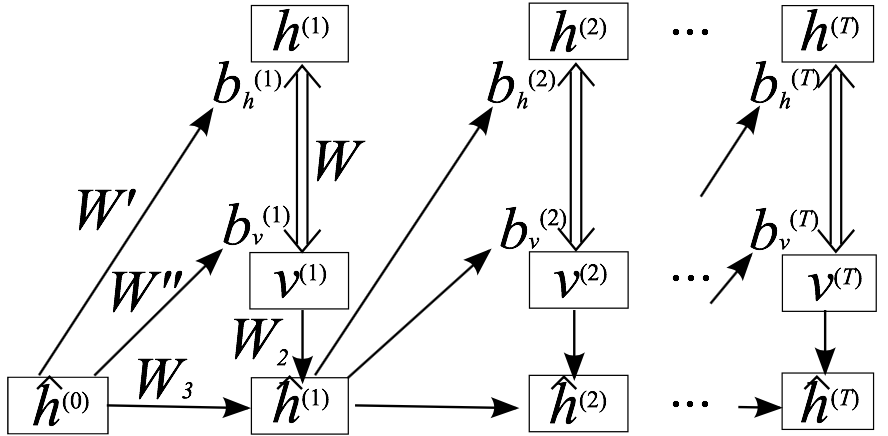
\includegraphics[scale=0.35]{rnnrbm.png}
      \caption{RNN-RBM (src: \cite{c8})}
      \label{fig:rnnrbm}
\end{figure}

In this project. the RTRBM and the RNNRBM are used to model the high-dimensional data and learn the probability distribution with a temporal setting. Each frame of the audio file is a time slices and the probabilities are learned by the RBM.

%%%%%%%%%%%%%%%%%%%%%%%%%%%%%%%%%%%%%%%%%%%%%%%%%%%%%%%%%%%%%%%
%%%%%%%%%%%%%%%%%%%%%%%%%%%%%%%%%%%%%%%%%%%%%%%%%%%%%%%%%%%%%%%
\section{Convolutional Dbn} 
Convolutional DBN (CDBN) consists of several max-pooling Convolutional RBMs (CRBM). A CRBM is similar to an RBM but the weights between the hidden layer and the visible layers are shared among all the locations (fully connected nature of RBM). An example can be seen in \ref{fig:crbm}. The basic CRBM contains two layers: a visible input layer $V$ and a hidden layer $H$. The input layer consists of a mesh of $N_V \times N_V$ array of binary units. The hidden layer consists of $K$ groups of $N_H \times N_H$ units, thus a total of $N_H^2 K$ units. Similar to a traditional RBM, one can perform block Gibbs sampling using the specific conditions as detailed in \cite{c12}.

Coming back to CDBN, the architecture consists of several max-pooling-CRBMs stacked on top of one another, analogous to DBNs. The network defines an energy function by summing the energy functions for all the individual pairs of layers.
\begin{figure}[thpb]
      \centering
      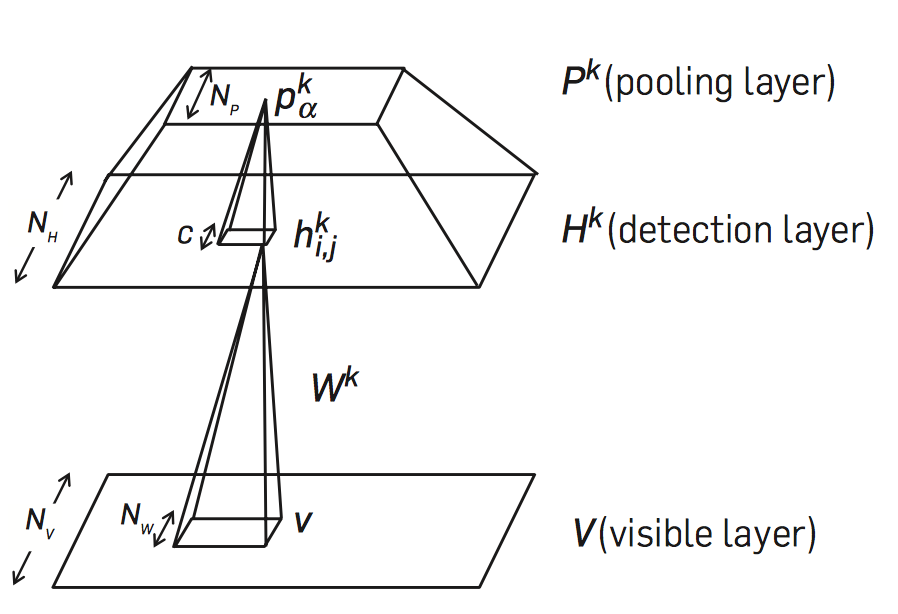
\includegraphics[scale=0.55]{crbm.png}
      \caption{Convolutional RBM with probabilistic max-pooling.(src: \cite{c12})}
      \label{fig:crbm}
\end{figure}

In the project, the use of CDBN was to form a convoluted structure on top of chroma and STFT representations of the audio file as displayed in Fig: \ref{fig:mel} and Fig: \ref{fig:choma}. The implementation of the 

\section{Datasets}
The datasets that were used for the experiments were: (1) A collection of low-level features of audio files created from a collection of MPEG-3 files using the LibROSA library \cite{c0}. The features were STFT, Spectrogram, MFCC. (2)  Nottingham dataset\footnote{\tt{http://ifdo.ca/\texttildelow{seymour}/nottingham/nottingham.html}}: It is a collection of 1200 folk tunes with chords instantiated from the Notes(ABC) format with 7 hours of polyphonic music. The polyphony (number of simultaneous notes) varies from 0 to 15 and the average polyphony is 3.9. (3) MAPS dataset\footnote{\url{http://tinyurl.com/maps-dataset}}: 6 piano files, with nearly thirty minutes of music. Test data comprised of 4 files with nearly 15 minutes of music. (2) and (3) are collection of midi file collections. 

\section{Experiments and Results}
The implementation of the the experiments was done in different parts. The audio feature extraction, as shown in Fig. \ref{fig:spectral}, was done using NumPy, SciPy and LibROSA library \cite{c0} in Python. For training RNN-RBM I have used the implementation given on \url{www.deeplearning.net}. The implementation uses Stochastic Gradient Descent on every time step for updating parameters. Contrastive Divergence is used in Stochastic Gradient Descent for Gibbs sampling. Instead of random sampling Contrastive Divergence uses the distribution of training data for sampling which leads to faster convergence. I trained the model on 200 epochs for learning the features. The implementation of RNN-RBM is done in Theano with the code for MIDI processing and the transcription present in the authors webpage\cite{c8}. The implementation of CDBN could not be completely done by me as the modules required for the DBN processing in PyLearn2 were not present. A MATLAB implementation for CDBN for MNIST dataset was available on the webpage of the first author of \cite{c12}. This was modified to take audio and pickle files as an input. The learned results were not readable by a Wave processor and could not be processed to see its success rate.

\begin{figure}[thpb]
      \centering
      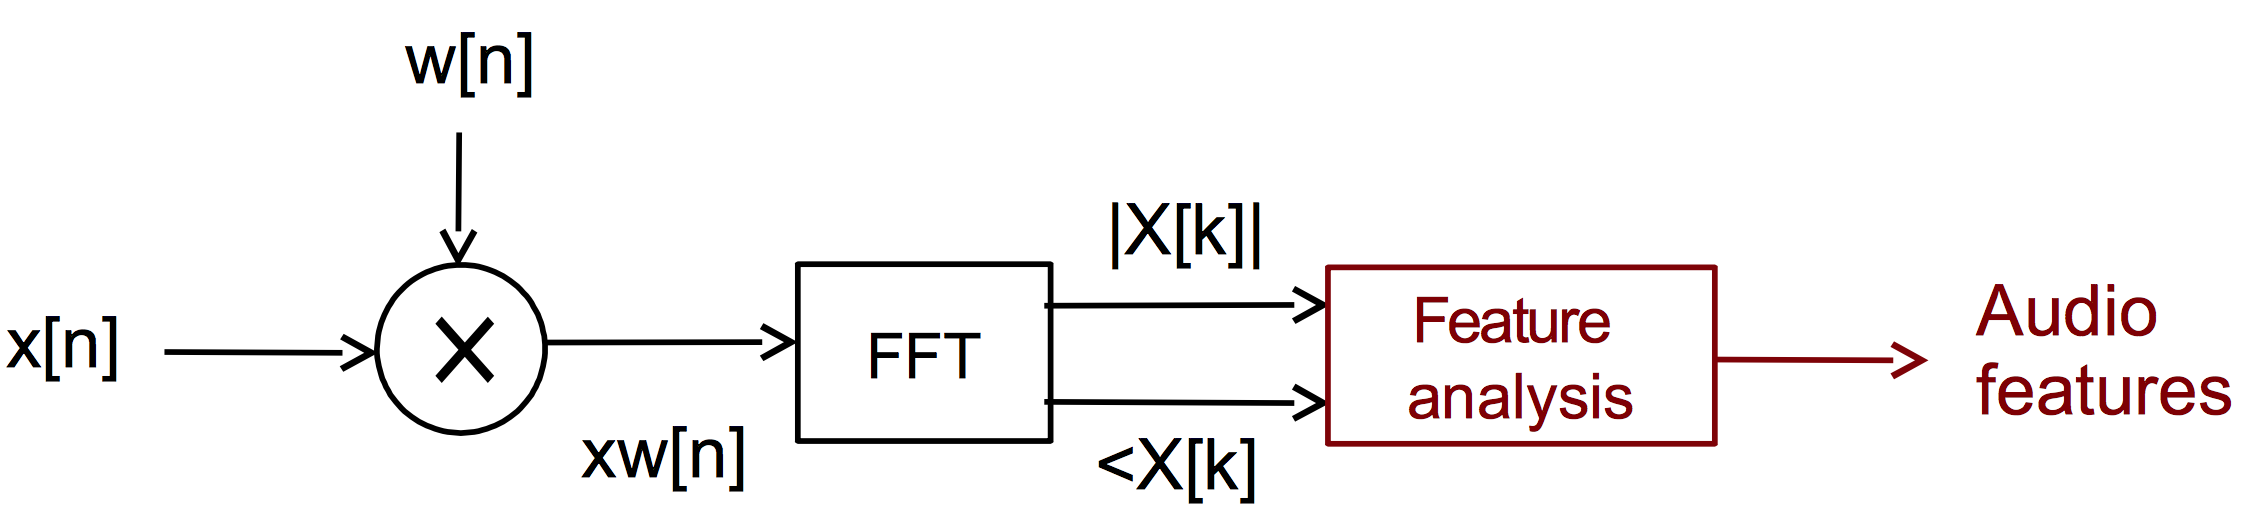
\includegraphics[scale=0.23]{spectral.png}
      \caption{Model to get the audio features.}
      \label{fig:spectral}
\end{figure}

\subsection{Application of RNNRBM to generate MIDI}
The training of the RNN-RBM implementation was done for multiple number of epochs on the Nottingham dataset. As the epochs increased, the temporal nature of the midi and notes helped the RBN to model the data better. As you can see, the Fig. \ref{fig:ex1} shows the midi transcribed after 4 epochs. The notes are constructed at random and not very stable. Whereas, Fig. \ref{fig:ex2}, which generate the MIDI after 200 epochs are far more stable and sound better as well. 

\begin{figure}[thpb]
      \centering
      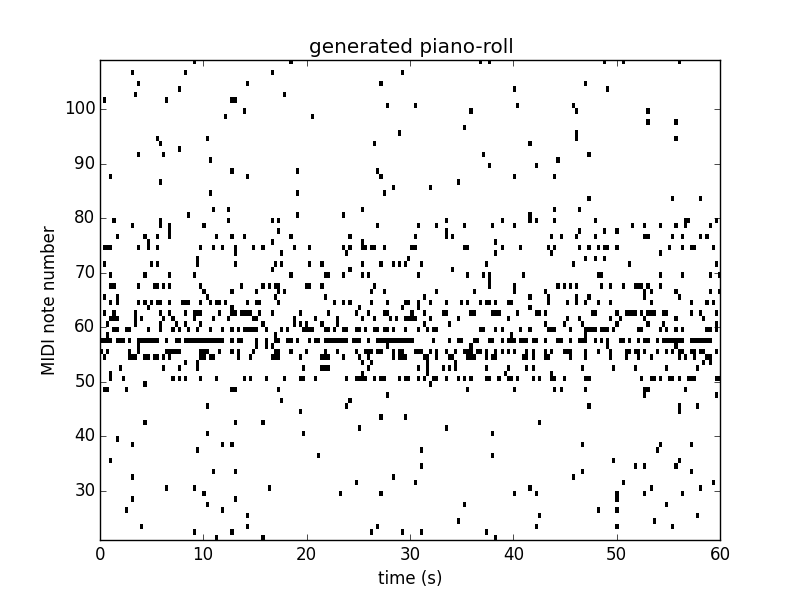
\includegraphics[scale=0.35]{epoch_1_1.png}
      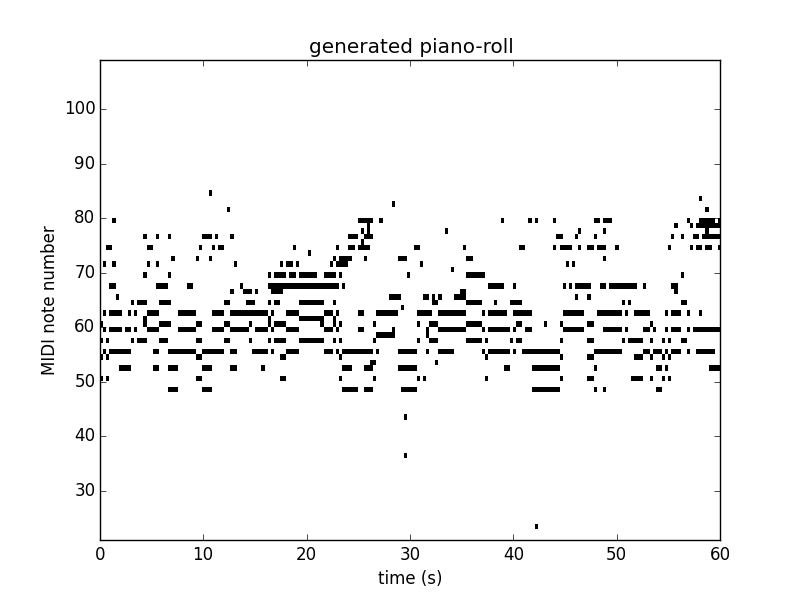
\includegraphics[scale=0.35]{epoch_200_1.png}
      \caption{Transcription of Midi, after 4 and 200 Epochs - Example 1}
      \label{fig:ex1}
\end{figure}
\begin{figure}[thpb]
      \centering
      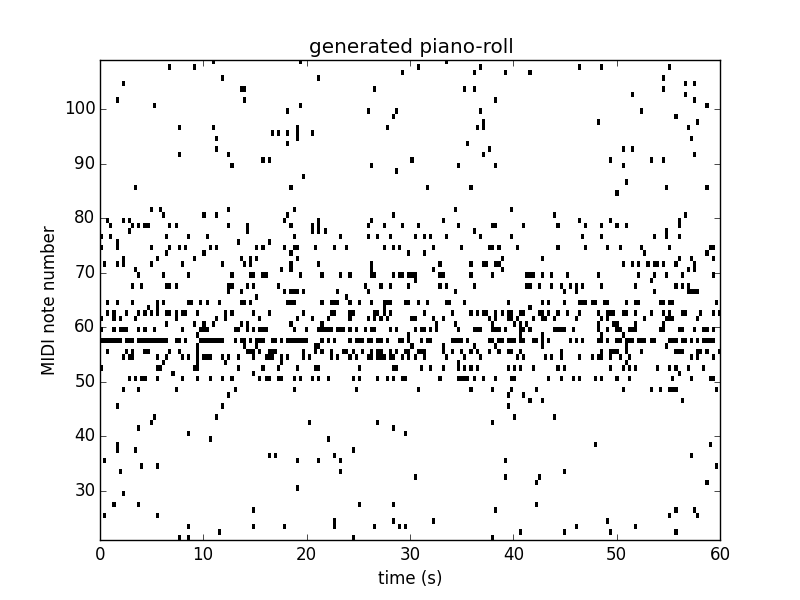
\includegraphics[scale=0.35]{epoch_1_4.png}
      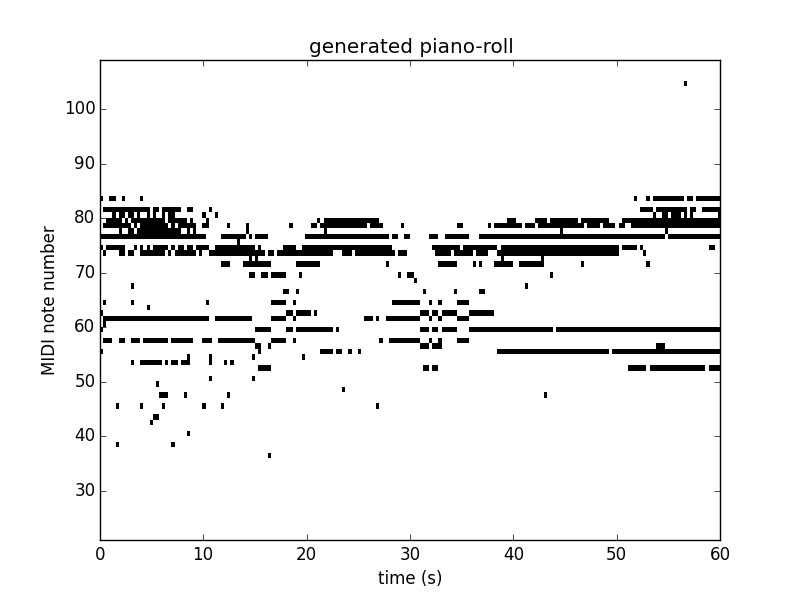
\includegraphics[scale=0.35]{epoch_200_4.png}
      \caption{Transcription of Midi, after 4 and 200 Epochs - Example 2}
      \label{fig:ex2}
\end{figure}

\subsection{Experiments with Indian Percussion Instruments}
I collected the dataset for Indian percussion instruments from different websites and learnt its features using RNN-RBM but the features learned were poor because of alignment problems in corresponding wav and midi files.

\section{Conclusion}
I was able to generate a simple digital audio file of midi file format using the RNN-RBM model. But using CDBN using on low-level features such as chroma and STFTs of the audio did not generate any music. I hope to be able to build a system based on the work done by Lee et. al.\cite{c1} and extend it for music generation based on audio features, in the future.

\addtolength{\textheight}{-12cm}  

\section*{ACKNOWLEDGMENT}
I would like to thank Prof. Baldi for introducing me to the world of Deep Learning and making us better students in in the process.

\begin{thebibliography}{99}
\bibitem{c0} B. McFee, M. McVicar, C. Raffel, D. Liang, and Douglas Repetto, \textit{librosa: v0.3.1.}, ZENODO, 2014.
\bibitem{c1} H. Lee, P. Pham, Y. Largman, and A. Y. Ng. \textit{Unsupervised feature learning for audio classification using convolutional deep belief networks.}, In Advances in neural information processing systems, pp. 1096--1104. 2009.
\bibitem{c2} V. Emiya, R. Badeau, and B. David. \textit{Multipitch estimationof piano sounds using a new probabilistic spectral smoothness principle}, IEEE Transactions on Audio, Speech, and Language Processing, 18.6, pp. 1643--1654. 2010.
\bibitem{c3} G. Peeters. \textit{A large set of audio features for sound description (similarity and classification) in the cuidado project.}, Technical report, IRCAM, 2004
\bibitem{c4} T. Jehan. \textit{Creating music by listening.}, PhD diss., Massachusetts Institute of Technology, 2005. \url{http://web.media.mit.edu/~tristan/phd/}
\bibitem{c5} H. Cohen, \textit{The further exploits of AARON, painter.}, Stanford Humanities Review 4, no. 2, pp. 141--158. 1995.
\bibitem{c6} R. Typke, F. Wiering, and R. C. Veltkamp. \textit{A Survey of Music Information Retrieval Systems.} In ISMIR, pp. 153--160. 2005.
\bibitem{c7} R. Demopoulos, and M. Katchabaw. \textit{Music Information Retrieval: A Survey of Issues and Approaches.} Vol. 677. Technical Report, 2007.
\bibitem{c8}  N. Boulanger-Lewandowski, Y. Bengio, and P. Vincent. \textit{Modeling temporal dependencies in high-dimensional sequences: Application to polyphonic music generation and transcription.}, Proceedings of the ICML-12, pp. 1159--1166 , 2012.
\bibitem{c9} G.E. Hinton, \textit{Training products of experts by minimizing contrastive divergence.}, Neural Computation, 14(8): 1771--1800, 2002.
\bibitem{c10} D. Eck, and J. Schmidhuber, \textit{Finding temporal structure in music: Blues improvisation with LSTM recurrent networks.}, In NNSP, pp. 747--756, 2002.
\bibitem{c11} J. Nam, J. Ngiam, H. Lee, and M. Slaney. \textit{A Classification-Based Polyphonic Piano Transcription Approach Using Learned Feature Representations.} In ISMIR, pp. 175-180. 2011.
\bibitem{c12} H. Lee, R. Grosse, R. Ranganath, and A. Y. Ng. \textit{Unsupervised learning of hierarchical representations with convolutional deep belief networks.} Commun. ACM 54, 10 (October 2011), 95-103. 2011.
\bibitem{c13} G.E. Hinton, S. Osindero, Y. W. Teh, \textit{A Fast Learning Algorithm for Deep Belief Nets.} Neural Comput. 18. 7, 1527--1554. 2006.
\bibitem{c13} I. Sutskever, G. E. Hinton, and G. W. Taylor. \textit{The recurrent temporal restricted boltzmann machine.} In Advances in Neural Information Processing Systems, pp. 1601--1608. 2009.
\end{thebibliography}

\pagebreak 
\section*{APPENDIX}
A description of Audio descriptors
\subsection{Some Spectral Descriptors}
\begin{itemize}
\item Spectral descriptors: Bark Bands, Mel Bands, ERB Bands, MFCC, GFCC, LPC, HFC, Spectral Contrast, In harmonicity and Dissonance, etc.
\item Time-domain descriptors: Effective Duration, ZCR, Loudness, etc.
\item Tonal descriptors: Pitch Salience Function, Pitch Y-in FFT, HPCP, Tuning Frequency, Key, Chords Detection, etc.
\item Rhythm descriptors: Beat Tracker Degara, Beat Tracker Multi Feature, BPM Histogram Descriptors, Novelty Curve, Onset Detection, Onsets, etc.
\item SFX descriptors: Log Attack Time, Max To Total, Min To Total, TC To Total, etc.
\item High-level descriptors: Danceability, Dynamic Complexity, Fade Detection, etc.
\end{itemize}

\subsection{Some Single-frame spectral features}
\begin{itemize}
\item Energy, RMS, Loudness
\item Spectral centroid
\item Mel-frequency cepstral coefficients (MFCC)
\item Pitch salience
\item Chroma (Harmonic pitch class profile, HPCP)
\end{itemize}

\end{document}
